\subsection{Par\'ametros estructurales del $\mathbf{BiFeO_{3}}$ con arreglos 
antiferromagn\'eticos tipo A y G}

La tabla \ref{tabla_BiFeO3_parametro_red} muestra los par\'ametros 
estructurales (a, c) de la red hexagonal del $BiFeO_{3}$ en el espacio de grupo 
R3c (\#161) para los dos arreglos antiferromagn\'eticos. Los par\'ametros se 
obtuvieron de la relajaci\'on de la estructura cristalina. Los valores 
obtenidos se encuentran en concordancia con resultados experimentales 
\cite{lu2010}, y te\'oricos obtenidos con DFT 
\cite{lee2012,arnold2015}.

% ------------------------------
% TABLA: parametros optimizados
% ------------------------------

\begin{table}[H]
    \begin{center}
        \caption[Par\'ametros de red optimizados del 
        $BiFeO_{3}$]{Comparaci\'on 
            de los par\'ametros estructurales de los dos arreglos 
            antiferromagn\'eticos, con valores obtenidos de 
            difracci\'on de 
            rayos X y DFT}
        \begin{tabular}{ccc}
            \hline
                 & \textbf{a (\AA)} & \textbf{c (\AA)} \\
            \hline \hline
            AF-A & $5.65$ & $14.16$ \\
            \hline
            AF-G & $5.64$ & $14.07$ \\
            \hline
            \cite{lu2010} & $5.58$ & $13.90$ \\
            \hline
            \cite{lee2012} & $5.6143$ & $13.98$ \\
            \hline
            \cite{arnold2015} & $5.5725$ & $13.85$ \\
            \hline
        \end{tabular}
        \label{tabla_BiFeO3_parametro_red}
    \end{center}
\end{table}

\noindent Los par\'ametros estructurales de menor valor pertenecen al arreglo 
antiferromagn\'etico tipo G, y la tabla 
\ref{tabla_BiFeO3_ener_vol_mag} muestra 
que 
posee la menor energ\'ia total y el menor volumen. Por lo tanto el 
arreglo 
antiferromagn\'etico tipo G es el m\'as estable.

% 
%------------------------------------------------------------------------
% TABLA: energia total, volumen de la celda, momento magnetico del 
%hierro
% 
%------------------------------------------------------------------------

\begin{table}[H]
    \begin{center}
        \caption{Energ\'ia total, volumen de la celda y momento 
            magn\'etico del 
            \'atomo de hierro,
            para el $BiFeO_{3}$ con los arreglos antiferromagn\'eticos tipo A y 
            G}
        \begin{tabular}{cccc}
            \hline
            \textbf{Tipo} & \textbf{Energ\'ia total (Ry)} & 
            \textbf{Volumen 
                (\AA $^{3}$)} & \textbf{Momento magn\'etico Fe ($\mu 
                _{B}$)}\\
            \hline \hline
            AF-A & $-3194.656$ & $391.58$ & $4.19$ \\
            \hline
            AF-G & $-3194.725$ & $387.55$ & $4.05$ \\
            \hline
        \end{tabular}
        \singlespace
        \label{tabla_BiFeO3_ener_vol_mag}
    \end{center}
\end{table}

\noindent Los momentos magn\'eticos del hierro de los dos arreglos 
antiferromagn\'eticos 
mostrados en la tabla \ref{tabla_BiFeO3_ener_vol_mag} se encuentran en 
concordancia con los datos experimentales de $3.75$ $\mu _{B}$ 
\cite{fischer1980} 
y $4.0$ $\mu _{B}$ \cite{sosnowska2002}. Las diferencias entre los resultados 
obtenidos y los datos experimentales pueden ser atribuidos a varios factores, 
tales como temperatura y posibles defectos de formaci\'on en las muestras de 
$BiFeO_{3}$ y en el caso de los datos obtenidos con DFT, puede deberse a como 
se encuentra implementado el m\'etodo de DFT + U en los distintos paquetes de 
simulaci\'on utilizados en dichos estudios.

\subsection{Estructura de bandas de energ\'ia del $\mathbf{BiFeO_{3}}$ con 
arreglo antiferromagn\'etico tipo A}

% ###########################################################
% ###########################################################
%                  INICIO TIPO A
% ###########################################################
% ###########################################################

% ----------------------------
% FIGURA: banda BiFeO3 tipo A
% ----------------------------

\begin{figure}[H]
    \centering
    
    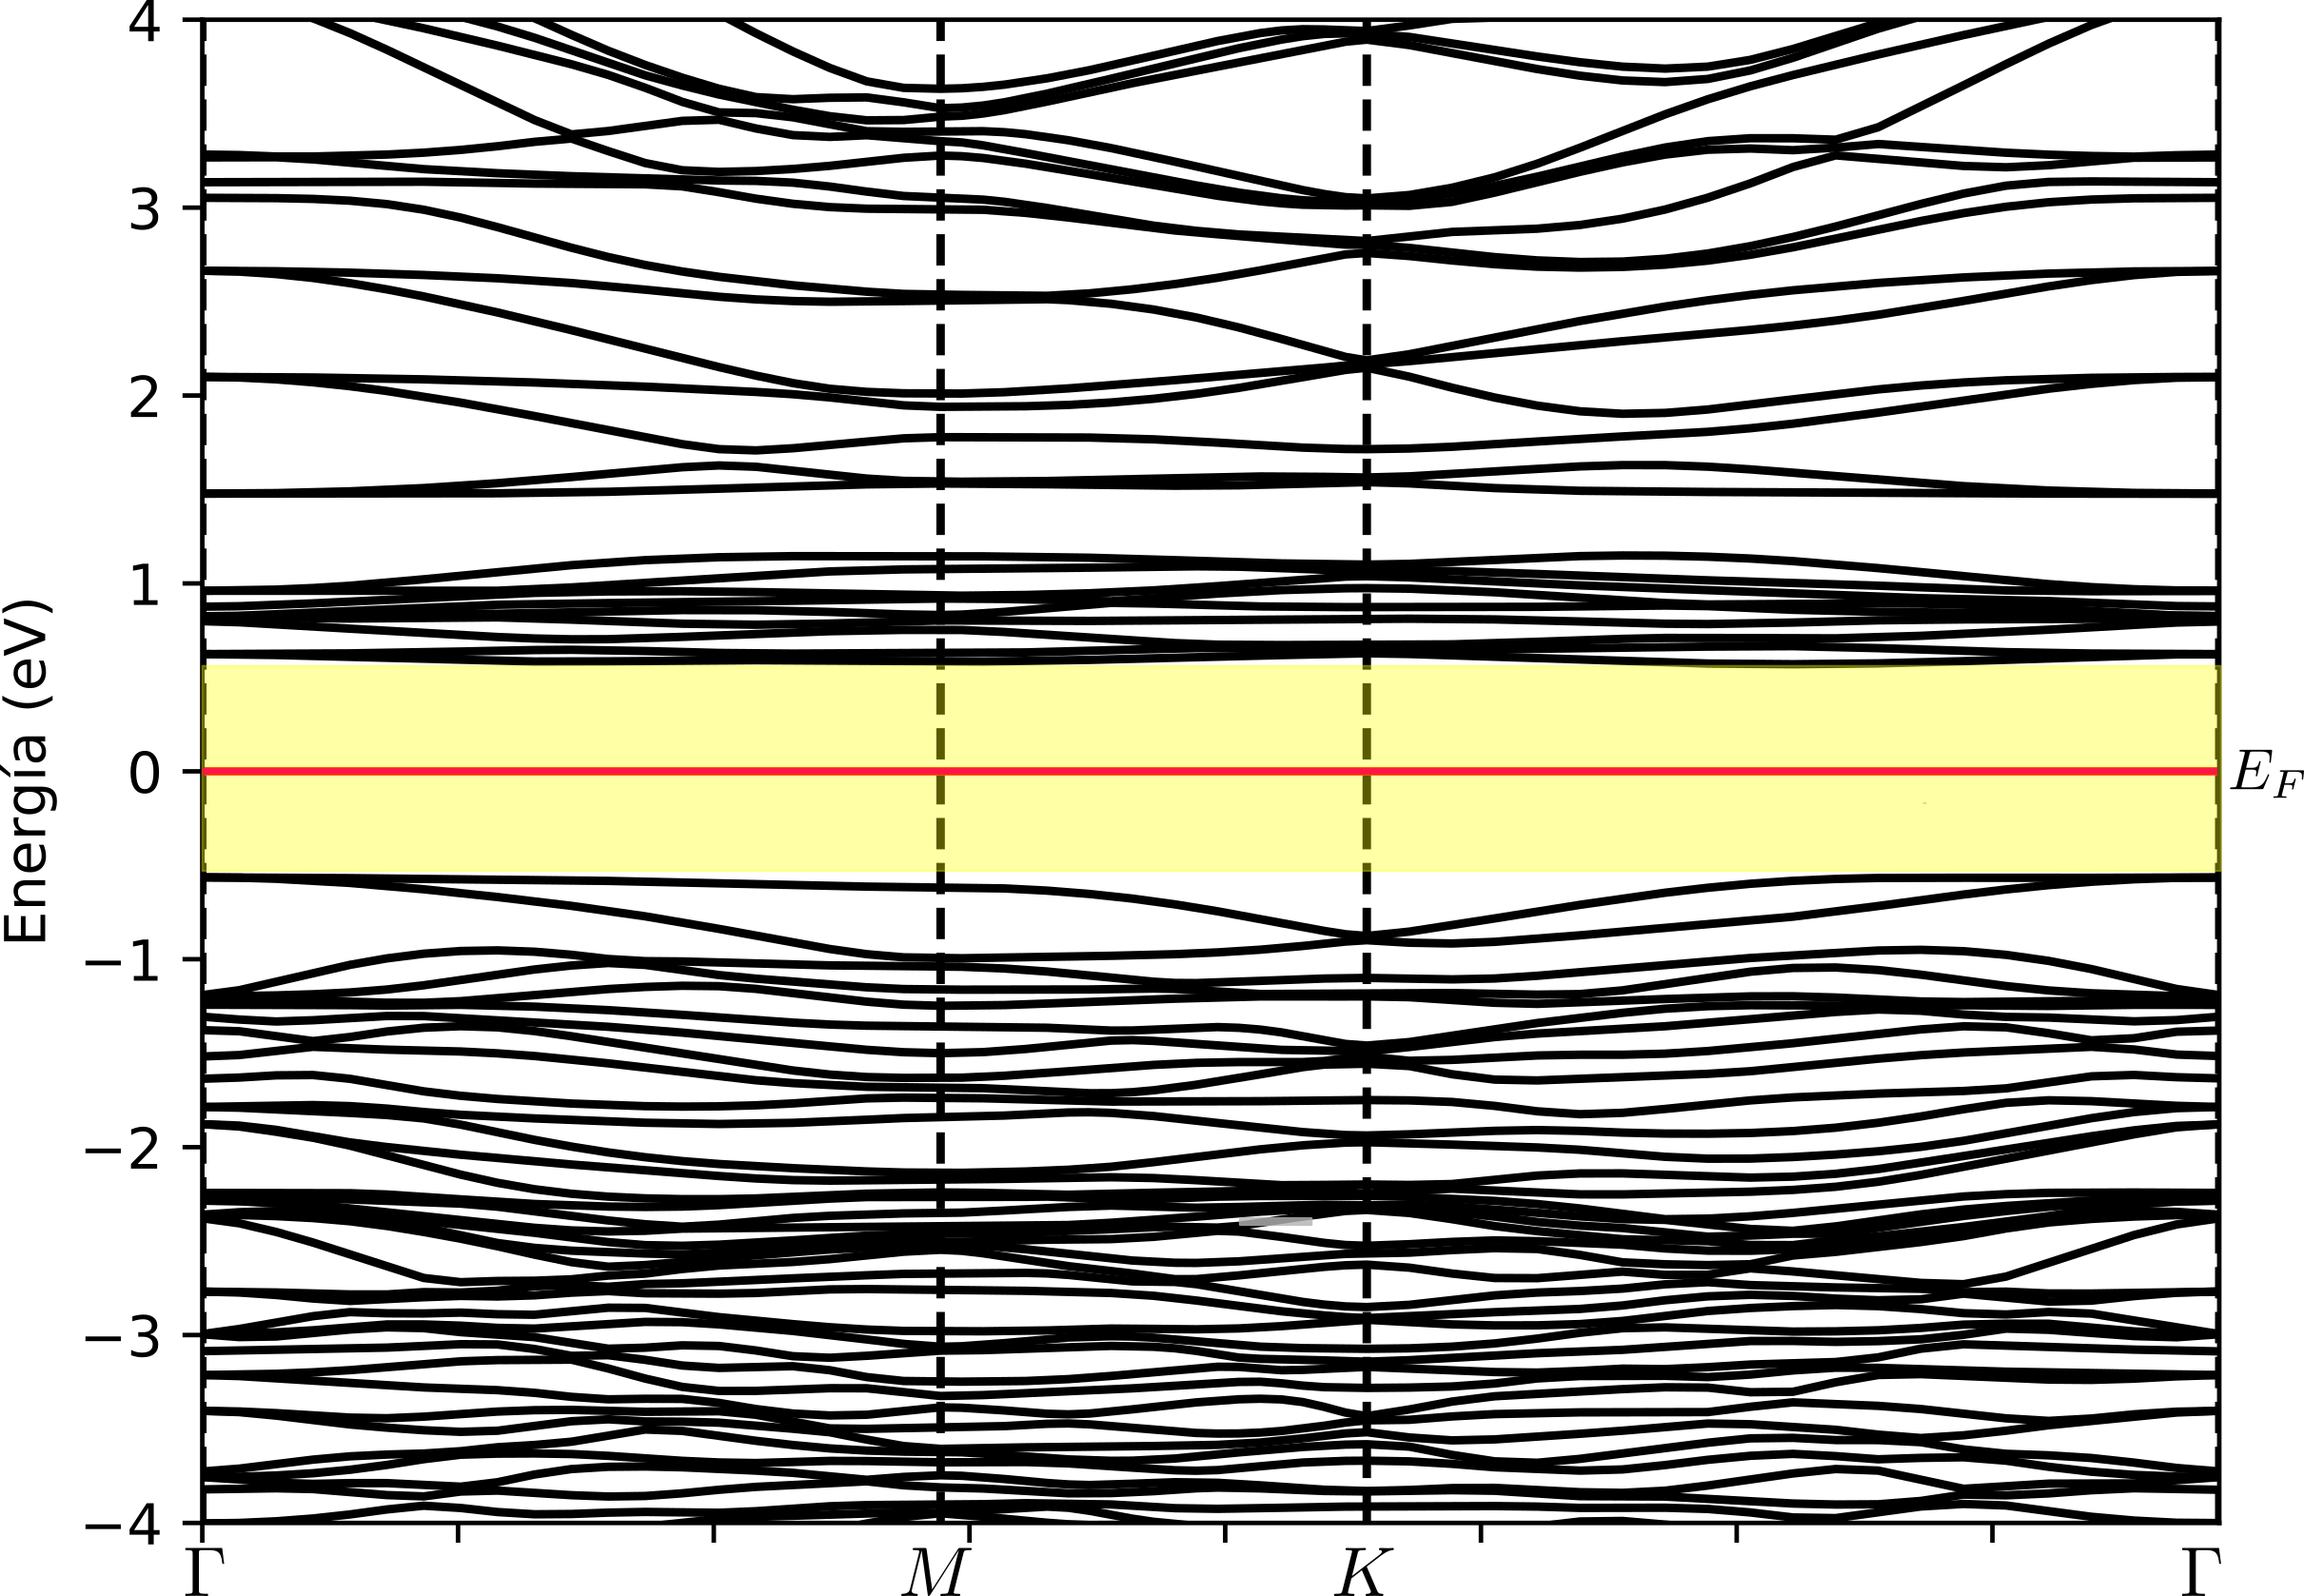
\includegraphics[width=0.7\textwidth]{contenido/resultados/ferrita_bismuto/img_ferrita_bismuto/BiFeO3_bandas_A_inf.png}
    \singlespace
    \caption[Bandas de energ\'ia del $BiFeO_{3}$ con arreglo 
    antiferromagn\'etico tipo A]{Estructura de bandas de energ\'ia del 
        $BiFeO_{3}$ con arreglo antiferromagn\'etico tipo A. La l\'inea roja 
        marca el 
        nivel de fermi. Los puntos de alta simetr\'ia tomados en la primera 
        zona de 
        brillouin son $\Gamma - M - K - \Gamma$.}
    \label{bfo_band_a}
\end{figure}

En la figura \ref{bfo_band_a} se observan las bandas de energ\'ia del arreglo 
antiferromagn\'etico tipo A del $BiFeO_{3}$. Las energ\'ias fueron escaladas 
respecto al nivel de fermi, que es tomado como el cero de la escala vertical. 
La estructura de bandas muestra un 
gap de 
energ\'ia alrededor del nivel de fermi, definido entre el nivel de energ\'ia 
m\'as alto de la banda de valencia ubicado en el punto $\Gamma$ y el nivel de 
energ\'ia m\'as bajo de la banda de conducci\'on ubicado entre los puntos $K - 
\Gamma$. El gap de energ\'ia es de $1.4$ eV el cual es cercano al valor de 
$1.3$ eV 
reportado por otros estudios \cite{ju2009,gujar2007}. En la banda de 
conducci\'on se observa una secci\'on alrededor del nivel de energ\'ia de $1.5$ 
eV que no posee bandas; de esta forma se pueden distinguir dos grupos de 
bandas. El grupo m\'as cercano al nivel de fermi es bastante denso, y el m\'as 
alejado no tanto. La banda de valencia en contraste es compacta.

\subsection{Densidad de estados del $\mathbf{BiFeO_{3}}$ con arreglo 
antiferromagn\'etico tipo A}

% -------------------------------------------
% FIGURA: densidades de estado BIFeO3 tipo G
% -------------------------------------------

\begin{figure}
    \centering
    \subfloat[]{
        \label{bfo_tot_a}
        
        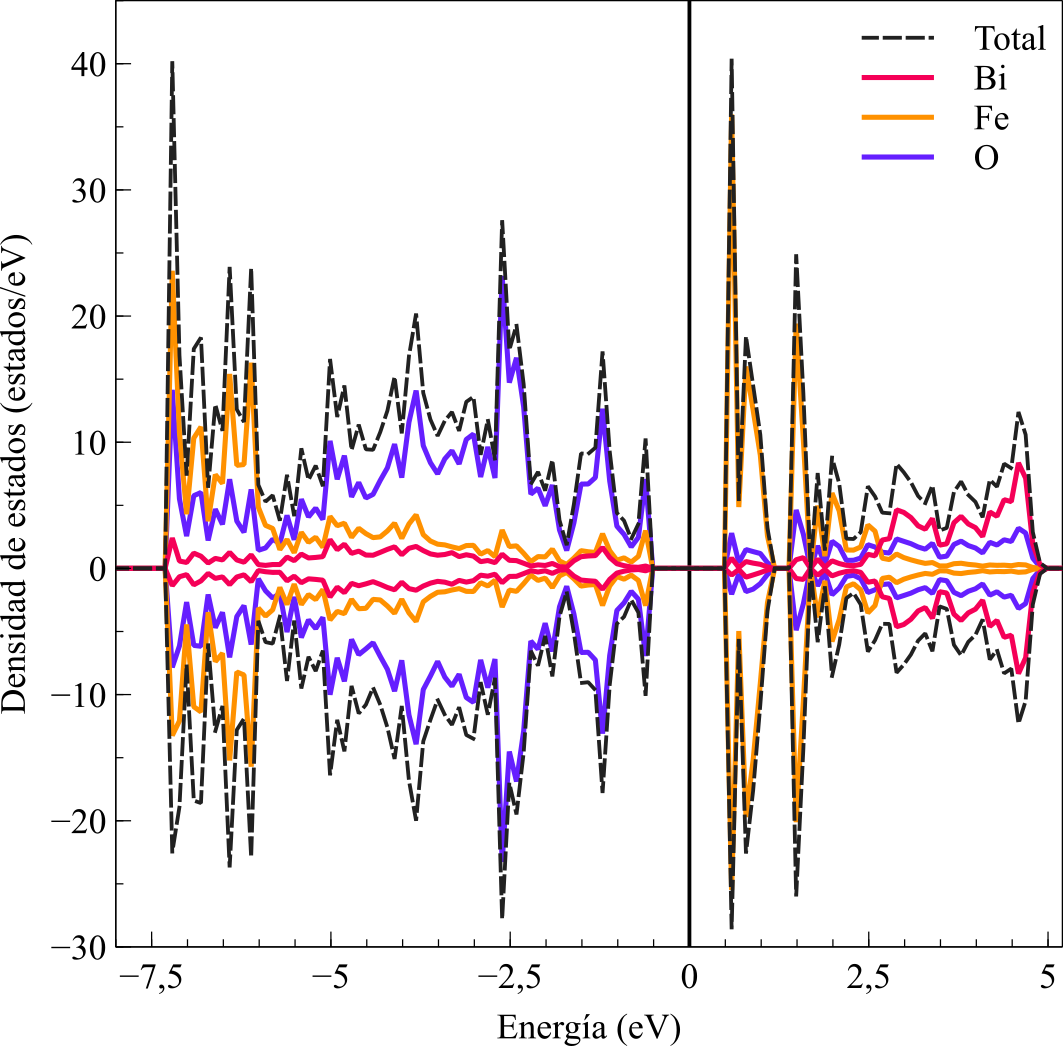
\includegraphics[width=0.5\textwidth]{contenido/resultados/ferrita_bismuto/img_ferrita_bismuto/BiFeO3_DOS_A_inf.png}}
    \subfloat[]{
        \label{bfo_bi_a}
        
        \includegraphics[width=0.5\textwidth]{contenido/resultados/ferrita_bismuto/img_ferrita_bismuto/BiFeO3_DOS_Bi_A_inf.png}}
    
    \subfloat[]{
        \label{bfo_fe_a}
        
        \includegraphics[width=0.5\textwidth]{contenido/resultados/ferrita_bismuto/img_ferrita_bismuto/BiFeO3_DOS_Fe_A_inf.png}}
    \subfloat[]{
        \label{bfo_o_a}
        
        \includegraphics[width=0.5\textwidth]{contenido/resultados/ferrita_bismuto/img_ferrita_bismuto/BiFeO3_DOS_O_A_inf.png}}
    \singlespace
    \caption[Densidad de estados del $BiFeO_{3}$ con arreglo 
    antiferromagn\'etico tipo A]{Densidad de estados del $BiFeO_{3}$ 
    con 
        arreglo antiferromagn\'etico tipo A. La linea negra en cero 
        indica el 
        nivel 
        de fermi. \ref{bfo_dos_a} \subref{bfo_tot_a} Densidad de estados total 
        y de cada elemento. 
        \ref{bfo_dos_a} \subref{bfo_bi_a} 
        Densidad de 
        estados para los orbitales s, p, d del bismuto. \ref{bfo_dos_a} 
        \subref{bfo_fe_a} Densidad 
        de estados 
        para los orbitales s, p ,d del hierro. \ref{bfo_dos_a} \subref{bfo_o_a} 
        Densidad de estados 
        para los 
        orbitales s, p del ox\'igeno.}
    \label{bfo_dos_a}
\end{figure}

% mmmmmmmmmmmmmmmmmmmmmmmmmmmmmmmmmmmmmmmmmmmmmmmmmmmmmmmmmmmmmmmm
%mmmmmmmmmmmmmmmmmmmmmmmmmmmmmmmmmmmmmmmmmmmmmmmmmmmmmmmmmmmmmmmmmmm
%mmmmmmmmmmmmmmmmmmmmmmmmmmmmmmmmmmmmmmmmmmmmmmmmmmmmmmmmmmmmmmmmmmmmm



La figura \ref{bfo_dos_a} \subref{bfo_tot_a} muestra la densidad de estados 
total para cada 
elemento que compone el $BiFeO_{3}$.Las energ\'ias fueron escaladas respecto al 
nivel de fermi que se tomo como cero de la escala horizontal, y la escala 
vertical positiva y negativa corresponden a los espines up y down 
respectivamente. En la banda de conducci\'on cerca del 
nivel de fermi observamos una densidad total de aproximadamente 40 estados/eV 
formada en su mayor\'ia por estados del hierro, seguida de peque\~nas 
contribuciones de bismuto y oxigeno. Tambi\'en podemos observar una secci\'on 
donde no existen estados de ning\'un elemento seguida de una densidad total de 
aproximadamente 25 estados/eV principalmente de hierro, seguido de oxigeno y 
bismuto. A partir del nivel de energ\'ia de 2 eV la densidad de estados total 
cae por debajo de 10 estados/eV , siendo el hierro dominante en el rango de 
2 eV a $2.5$ eV, pasado este nivel los estados de hierro son casi inexistentes, 
y 
el bismuto pasa a predominar manteniendo una densidad de estados por debajo de 
los 5 estados/eV hasta el nivel de 4 eV y elev\'andose hasta aproximadamente 8 
estados/eV alrededor de los $4.5$ eV.Por su parte la densidad de estados del 
oxigeno se mantiene por debajo de los 5 estados/eV sin cambios grandes. 
En la banda de valencia hasta el nivel de energ\'ia de -5 eV los estados de 
oxigeno poseen la mayor densidad de estados totales, fluctuando entre 5 
estados/ev y 25 estados/eV, y por debajo de los 5 estados/eV en el mismo rango 
de energ\'ia se encuentran estados de hierro seguidos por estados de bismuto. A 
partir de los -5 eV la densidad de estados de hierro supera a los otros 
elementos alcanzando aproximadamente los 25 estados/eV en su punto m\'as alto 
en el nivel de -7 eV seguido por los estados de oxigeno que se encuentran entre 
2 estados/eV y 15 estados/eV; y los estados de bismuto poseen una densidad de 
estados por debajo de 3 estados/eV.

% ===============================================
% ===============================================

\noindent La figura \ref{bfo_dos_a} \subref{bfo_bi_a} muestra la densidad de 
estados parcial del 
bismuto 
para cada uno de los orbitales \textbf{s}, \textbf{p} y \textbf{d}. Las 
energ\'ias fueron escaladas respecto al 
nivel de fermi que se tomo como cero de la escala horizontal, y la escala 
vertical positiva y negativa corresponden a los espines up y down 
respectivamente. En la banda 
de conducci\'on hasta el  nivel de energ\'ia de $2.5$ eV la densidad de estados 
se encuentra por debajo de 2 estados/eV y esta formada principalmente 
por el orbital \textbf{p} siendo casi inexistentes los orbitales \textbf{s} y 
\textbf{d}. A partir del nivel de energ\'ia de $2.5$ eV la densidad de estados 
fluct\'ua entre 2 estados/eV y 8 estados/eV, encontr\'andose su punto m\'as 
alto cerca del nivel de energ\'ia de 5 eV; en este rango de energ\'ia el 
orbital \textbf{p} sigue siendo el que m\'as contribuye en comparaci\'on a los 
orbitales \textbf{s} y \textbf{d}. En la banda de valencia se observa que hasta 
el nivel de energ\'ia de -2 eV el orbital \textbf{s} es el de mayor densidad, 
seguido por el orbital \textbf{p}, y la densidad de los orbitales \textbf{d} es 
pr\'acticamente cero. A partir del nivel de energ\'ia de $-2.5$ eV la densidad 
del orbital \textbf{p} pasa a ser la m\'as alta, alcanzando su m\'aximo en el 
nivel de enrg\'ia de $-7.5$ eV con 2 estados/eV. Adem\'as se puede observar que 
en el nivel de energ\'ia de -6 eV las densidades de estados de todos los 
orbitales se reducen casi a cero.

% -------------------------------------------------------------
% FIGURA: densidad de estado parcial hierro del BIFeO3 tipo A
% -------------------------------------------------------------

\noindent La figura \ref{bfo_dos_a} \subref{bfo_fe_a} muestra la densidad de 
estados parcial del 
hierro para 
cada uno de los orbitales \textbf{s}, \textbf{p} y \textbf{d}. Las energ\'ias 
fueron escaladas respecto al 
nivel de fermi que se tomo como cero de la escala horizontal, y la escala 
vertical positiva y negativa corresponden a los espines up y down 
respectivamente. En la banda de 
conducci\'on se observa que hasta el nivel de energ\'ia de 1 eV la densidad del 
orbital \textbf{d} es la m\'as alta alcanzando como m\'aximo los 35 estados/eV, 
y las densidades de los otros orbitales son casi inexistentes. A partir de 1 eV 
existe un peque\~no rango de energ\'ia donde las densidades de los orbitales 
son 
pr\'acticamente cero, luego de ese punto hasta el nivel de energ\'ia de $2.5$ 
eV 
la densidad del orbital \textbf{d} sigue siendo la m\'as alta, alcanzando como 
m\'aximo 20 estados/eV. A partir de los $2.5$ eV las densidades de los 
orbitales 
caen a cero. En la banda de valencia hasta el nivel de energ\'ia de $-5.5$ eV 
la 
densidad del orbital \textbf{d} es la m\'as alta manteni\'endose por debajo de 
4 estados/eV y las densidades de los otros orbitales son casi cero. A partir de 
$-5.5$ eV la densidad del orbital \textbf{d} sigue siendo la m\'as alta pero 
elev\'andose respecto al intervalo anterior, alcanzando su m\'aximo en $-7.5$ 
eV 
con 20 estados/eV, y los otros orbitales contin\'uan con una densidad casi 
inexistente.

% --------------------------------------------------------------
% FIGURA: densidad de estado parcial oxigeno del BIFeO3 tipo A
% --------------------------------------------------------------

\noindent La figura \ref{bfo_dos_a} \subref{bfo_o_a} muestra la densidad de 
estados parcial del 
ox\'igeno, 
para cada uno de los orbitales \textbf{s} y \textbf{p}. Las energ\'ias 
fueron escaladas respecto al 
nivel de fermi que se tomo como cero de la escala horizontal, y la escala 
vertical positiva y negativa corresponden a los espines up y down 
respectivamente. En la banda de conducci\'on se observa que hasta 
aproximadamente 1 eV la densidad del orbital \textbf{p} es la m\'as alta, 
estando por debajo de 2 estados/eV y la densidad del orbital \textbf{s} es casi 
inexistente. A partir de este punto existe un rango de energ\'ia corto donde 
las densidades de ambos orbitales son cero. Luego de este rango la densidad del 
estado \textbf{p} continua por sobre la del orbital \textbf{s} pero por debajo 
de 4 estados/eV. En la banda de valencia se observa que la densidad del orbital 
\textbf{p} es la m\'as alta y la densidad del orbital \textbf{s} es 
pr\'acticamente cero. La densidad del orbital \textbf{p} es de aproximadamente 
6 estados/eV alrededor del nivel de energ\'ia $-0.5$ eV , elev\'andose hasta 10 
estados/eV alrededor del nivel de energ\'ia de -1 eV, luego se reduce por 
debajo de 2 estados/eV cerca del nivel de -2 eV para luego alcanzar su m\'aximo 
con 22 estados/eV en el nivel de energ\'ia $-2.5$ eV. Pasado este punto se va 
reduciendo hasta alcanzar un m\'inimo de 2 estados/eV en el nivel de energ\'ia 
de -6 eV, y luego se eleva hasta alcanzar 12 estados/eV en $-7.5$ eV.


% ###########################################################
% ###########################################################
%                  INICIO TIPO G
% ###########################################################
% ###########################################################

\subsection{Estructura de bandas de energ\'ia del $\mathbf{BiFeO_{3}}$ con      
arreglo antiferromagn\'etico tipo G}

% ----------------------------
% FIGURA: banda BiFeO3 tipo G
% ----------------------------

\begin{figure}[H]
    \centering
    
    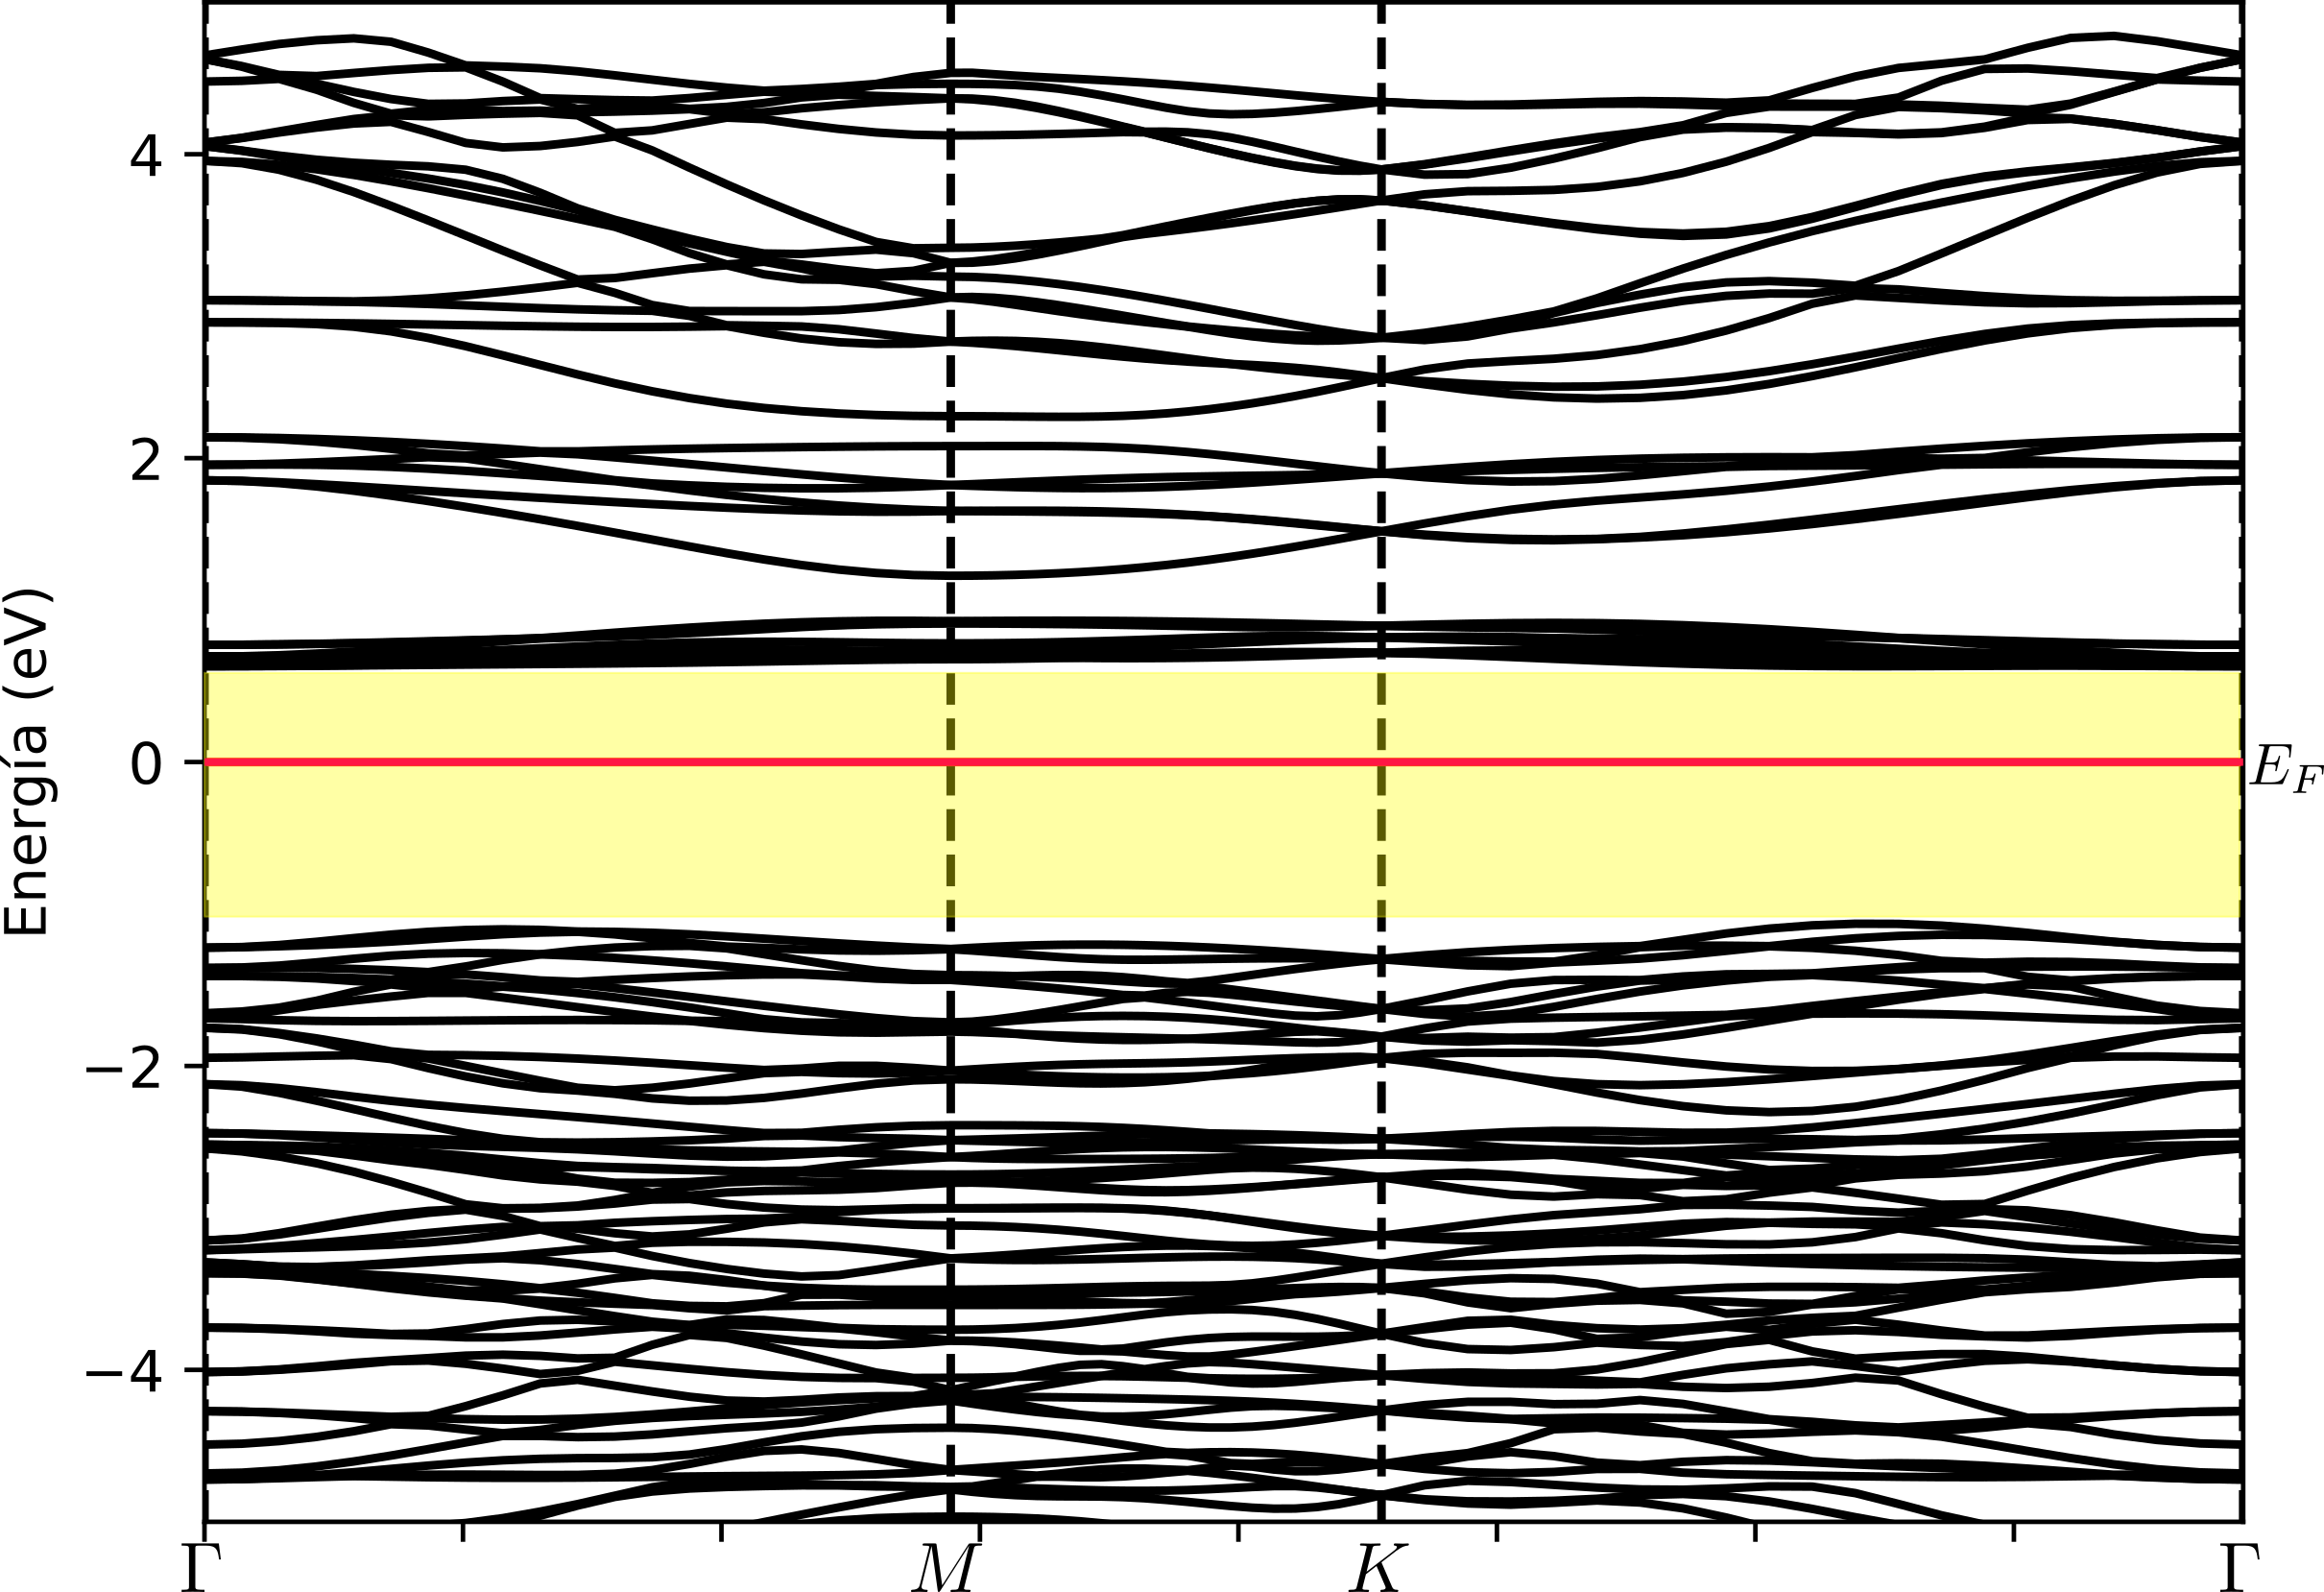
\includegraphics[width=0.7\textwidth]{contenido/resultados/ferrita_bismuto/img_ferrita_bismuto/BiFeO3_bandas_G_inf.png}
    \singlespace
    \caption[Bandas de energ\'ia del $BiFeO_{3}$ con arreglo 
    antiferromagn\'etico tipo G]{Estructura de bandas de energ\'ia del 
        $BiFeO_{3}$ con arreglo antiferromagn\'etico tipo G. La l\'inea roja 
        marca el 
        nivel de fermi. Los puntos de alta simetr\'ia tomados en la primera 
        zona de 
        brillouin son $\Gamma - M - K - \Gamma$.}
    \label{bfo_band_g}
\end{figure}


La figura \ref{bfo_band_g} muestra la estructura de bandas de energ\'ia del 
$BiFeO_{3}$ con arreglo antiferromagn\'etico tipo G. Las energ\'ias 
fueron escaladas respecto al nivel de fermi, que es tomado como el 
cero de la escala vertical. Se observa que el gap de 
energ\'ia es de $1.8$ eV el cual es cercano al valor de $1.9$ eV reportado por 
otros estudios \cite{ju2009,lee2012}. El gap se halla entre el m\'inimo de la 
banda de conducci\'on ubicado entre los puntos $K - \Gamma$ y el m\'aximo de la 
banda de valencia ubicado entre los puntos $K - \Gamma$. En la banda de 
conducci\'on se observa alrededor del nivel de energ\'ia de 1 eV una zona sin 
bandas de energ\'ia, de modo similar por sobre los 2 eV existe una zona muy 
estrecha que no presenta bandas de energ\'ia.

\subsection{Densidad de estados del $\mathbf{BiFeO_{3}}$ con arreglo      
antiferromagn\'etico tipo G}

% -------------------------------------------
% FIGURA: densidades de estado BIFeO3 tipo G
% -------------------------------------------

\begin{figure}[H]
    \centering
    \subfloat[]{
        \label{bfo_tot_g}
        
        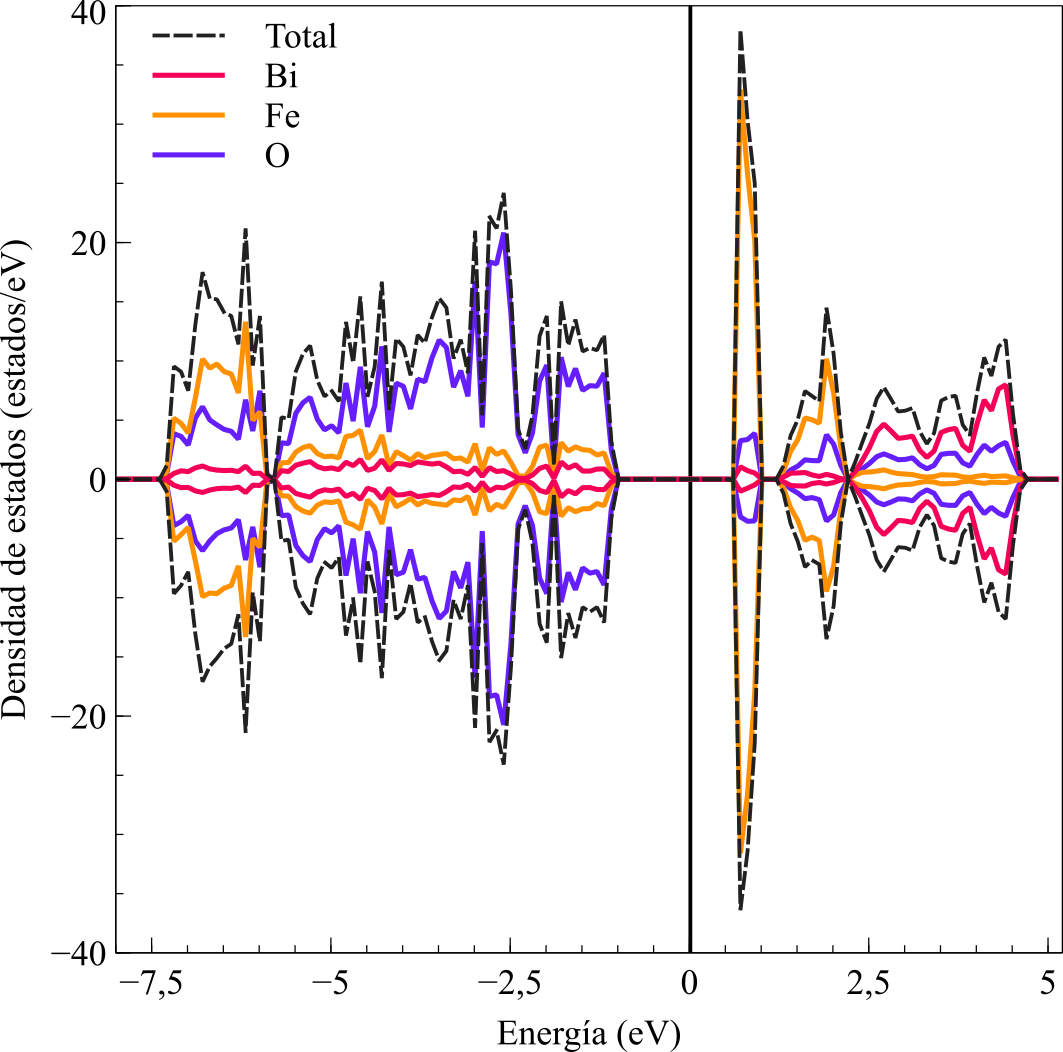
\includegraphics[width=0.5\textwidth]{contenido/resultados/ferrita_bismuto/img_ferrita_bismuto/BiFeO3_DOS_G_inf.png}}
    \subfloat[]{
        \label{bfo_bi_g}
        
        \includegraphics[width=0.5\textwidth]{contenido/resultados/ferrita_bismuto/img_ferrita_bismuto/BiFeO3_DOS_Bi_G_inf.png}}
    
    \subfloat[]{
        \label{bfo_fe_g}
        
        \includegraphics[width=0.5\textwidth]{contenido/resultados/ferrita_bismuto/img_ferrita_bismuto/BiFeO3_DOS_Fe_G_inf.png}}
    \subfloat[]{
        \label{bfo_o_g}
        
        \includegraphics[width=0.5\textwidth]{contenido/resultados/ferrita_bismuto/img_ferrita_bismuto/BiFeO3_DOS_O_G_inf.png}}
    \singlespace
    \caption[Densidad de estados del $BiFeO_{3}$ con arreglo 
    antiferromagn\'etico tipo G]{Densidad de estados del $BiFeO_{3}$ 
    con 
        arreglo antiferromagn\'etico tipo G. La linea negra en cero 
        indica el 
        nivel 
        de fermi. \ref{bfo_dos_g} \subref{bfo_tot_g} Densidad de estados total 
        y de cada elemento. 
        \ref{bfo_dos_g} \subref{bfo_bi_g} 
        Densidad de 
        estados para los orbitales s, p, d del bismuto. \ref{bfo_dos_g} 
        \subref{bfo_fe_g} Densidad 
        de estados 
        para los orbitales s, p ,d del hierro. \ref{bfo_dos_g} \subref{bfo_o_g} 
        Densidad de estados 
        para los 
        orbitales s, p del ox\'igeno.}
    \label{bfo_dos_g}
\end{figure}



% -------------------------------------------------------------
% FIGURA: densidad de estado total y por elemento del BIFeO3 tipo G
% -------------------------------------------------------------

\noindent La figura \ref{bfo_dos_g} \subref{bfo_tot_g} muestra la densidad de 
estados total para 
cada elemento que compone al $BiFeO_{3}$. Las energ\'ias fueron 
escaladas respecto al 
nivel de fermi que se tomo como cero de la escala horizontal, y la 
escala 
vertical positiva y negativa corresponden a los espines up y down 
respectivamente. En la banda de conducci\'on se observa que cerca al 
nivel de fermi los estados de hierro son los predominantes con una 
densidad de aproximadamente 40 estados/eV y con una densidad m\'as 
reducida se encuentran estados de ox\'igeno seguidos de estados de 
bismuto. En el rango de $1.5$ eV a $2.5$ eV los estados de hierro 
presentan una densidad por debajo de los 20 estados/eV y los estados 
de ox\'igeno y bismuto presentan densidades similares al intervalo 
anterior. A partir del nivel de energ\'ia de $2.5$ eV los estados de 
bismuto son los predominantes con una densidad aproximada de 5 
estados/eV mezclados con estados de ox\'igeno, en este rango de 
energ\'ia el hierro presenta una densidad de estados casi nula. En la 
banda de valencia, por debajo del nivel de fermi hasta el nivel de 
energ\'ia de $-5.5$ eV el ox\'igeno posee la mayor densidad de estados, 
seguido por los estados de hierro y bismuto con una baja densidad. 
A partir del nivel de energ\'ia de $-5.5$ eV el hierro posee la mayor 
densidad de estados con aproximadamente 15 estados/eV seguido por los 
estados de ox\'igeno con una densidad similar y el bismuto posee una 
densidad casi nula en este intervalo de energ\'ia.


% -------------------------------------------------------------
% FIGURA: densidad de estado parcial bismuto del BIFeO3 tipo G
% -------------------------------------------------------------

\noindent La figura \ref{bfo_dos_g} \subref{bfo_bi_g} muestra la densidad de 
estados parcial del 
bismuto 
para cada uno de los orbitales \textbf{s}, \textbf{p} y \textbf{d}. 
Las 
energ\'ias fueron escaladas respecto al 
nivel de fermi que se tomo como cero de la escala horizontal, y la 
escala 
vertical positiva y negativa corresponden a los espines up y down 
respectivamente. En la banda de conducci\'on cerca del nivel de fermi 
hasta el nivel de energ\'ia de aproximadamente $2.5$ eV se halla una 
densidad baja de estados de bismuto, siendo el orbital \textbf{p} el 
de mayor densidad y los otros dos orbitales presentan una densidad 
casi nula. A partir de $2.5$ eV la densidad de estados del orbital 
\textbf{p} aumenta considerablemente oscilando entre 5 estados/eV y 7 
estados/eV, en contraste las densidades de estado de los orbitales 
\textbf{s} y \textbf{d} son casi nulas, por lo que no contribuyen. En 
la banda de valencia cerca del nivel de fermi hasta los $-2.5$ eV el 
orbital \textbf{s} presenta la mayor densidad seguida por la densidad 
del estado \textbf{p}, siendo la densidad del orbital \textbf{d} casi 
nula. A partir del nivel de energ\'ia $-2.5$ eV hasta los $-7.5$ eV la 
densidad del orbital \textbf{p} vuelve a ser la mayor y los dem\'as 
orbitales presentan una densidad casi nula.

% -------------------------------------------------------------
% FIGURA: densidad de estado parcial hierro del BIFeO3 tipo G
% -------------------------------------------------------------

\noindent La figura \ref{bfo_dos_g} \subref{bfo_fe_g} muestra la densidad de 
estados parcial del 
hierro para cada uno de los orbitales \textbf{s}, \textbf{p} y 
\textbf{d}. 
Las 
energ\'ias fueron escaladas respecto al 
nivel de fermi que se tomo como cero de la escala horizontal, y la 
escala 
vertical positiva y negativa corresponden a los espines up y down 
respectivamente. En la banda de conducci\'on se observa que cerca del 
nivel de fermi y hasta aproximadamente 1 eV los estados del orbital 
\textbf{d} poseen una densidad de 30 estados/eV y los otros orbitales 
presentan una densidad casi nula,  dando luego paso a un peque\~no gap 
aproximadamente en $1.5$ eV. Luego hasta el nivel de energ\'ia de 
aproximadamente $2.5$ eV el orbital \textbf{d} sigue predominando con 
una densidad de 9 estados/eV y los dem\'as orbitales contin\'uan 
presentando una densidad casi nula. En la banda de valencia hasta 
aproximadamente el nivel de energ\'ia de $-5.5$ eV la densidad de 
estados del orbital \textbf{d} predomina y los dem\'as orbitales 
presentan una densidad casi nula, a partir de los $-5.5$ eV la densidad 
del orbital \textbf{d} aumenta hasta aproximadamente 10 estados/eV y 
los dem\'as orbitales contin\'uan teniendo una densidad bastante 
peque\~na.

% -------------------------------------------------------------
% FIGURA: densidad de estado parcial oxigeno del BIFeO3 tipo G
% -------------------------------------------------------------

\noindent La figura \ref{bfo_dos_g} \subref{bfo_o_g} muestra la densidad de 
estados parcial del 
hierro para cada uno de los orbitales \textbf{s} y \textbf{p}. 
Las 
energ\'ias fueron escaladas respecto al 
nivel de fermi que se tomo como cero de la escala horizontal, y la 
escala 
vertical positiva y negativa corresponden a los espines up y down 
respectivamente. En la banda de conducci\'on se observa que el orbital 
\textbf{p} presenta la mayor densidad de estados, aproximadamente 2 
estados/eV y los orbitales \textbf{s} presentan una densidad m\'as 
reducida. En la banda de valencia se observa un comportamiento 
similar, pero el orbital \textbf{p} presenta una mayor densidad de 
estados con un m\'aximo de 30 estados/eV aproximadamente en el nivel 
de energ\'ia $-2.5$ eV en contraste la densidad de estados del orbital 
\textbf{s} es casi nula.

\subsection{Densidad de carga del $\mathbf{BiFeO_{3}}$ con arreglos      
antiferromagn\'eticos tipo A y G}

La figura \ref{bfo_DC} muestra la densidad de carga de ambos arreglos 
antiferromagn\'eticos, con el fin de poder estudiar el tipo de enlace que 
existe entre los \'atomos de hierro y ox\'igeno, debido a que se pudo observar 
en la gr\'afica de densidad de estados un mezcla entre los estados de estos 
\'atomos. La densidad de carga entre el hierro y el ox\'igeno es 
aproximadamente $0.07$ e/\AA$^{3}$ lo que indica que la interacci\'on no es 
solo i\'onica sino que puede considerarse covalente. De manera similar la 
interacci\'on entre el bismuto y el ox\'igeno no es solo i\'onica dado que 
existe una densidad de carga de $0.04$ e/\AA$^{3}$. 


% ----------------------------
% FIGURA: densidades de carga
% ----------------------------

\begin{figure}
    \centering
    \subfloat[]{
        \label{bfo_DC_A}
        
        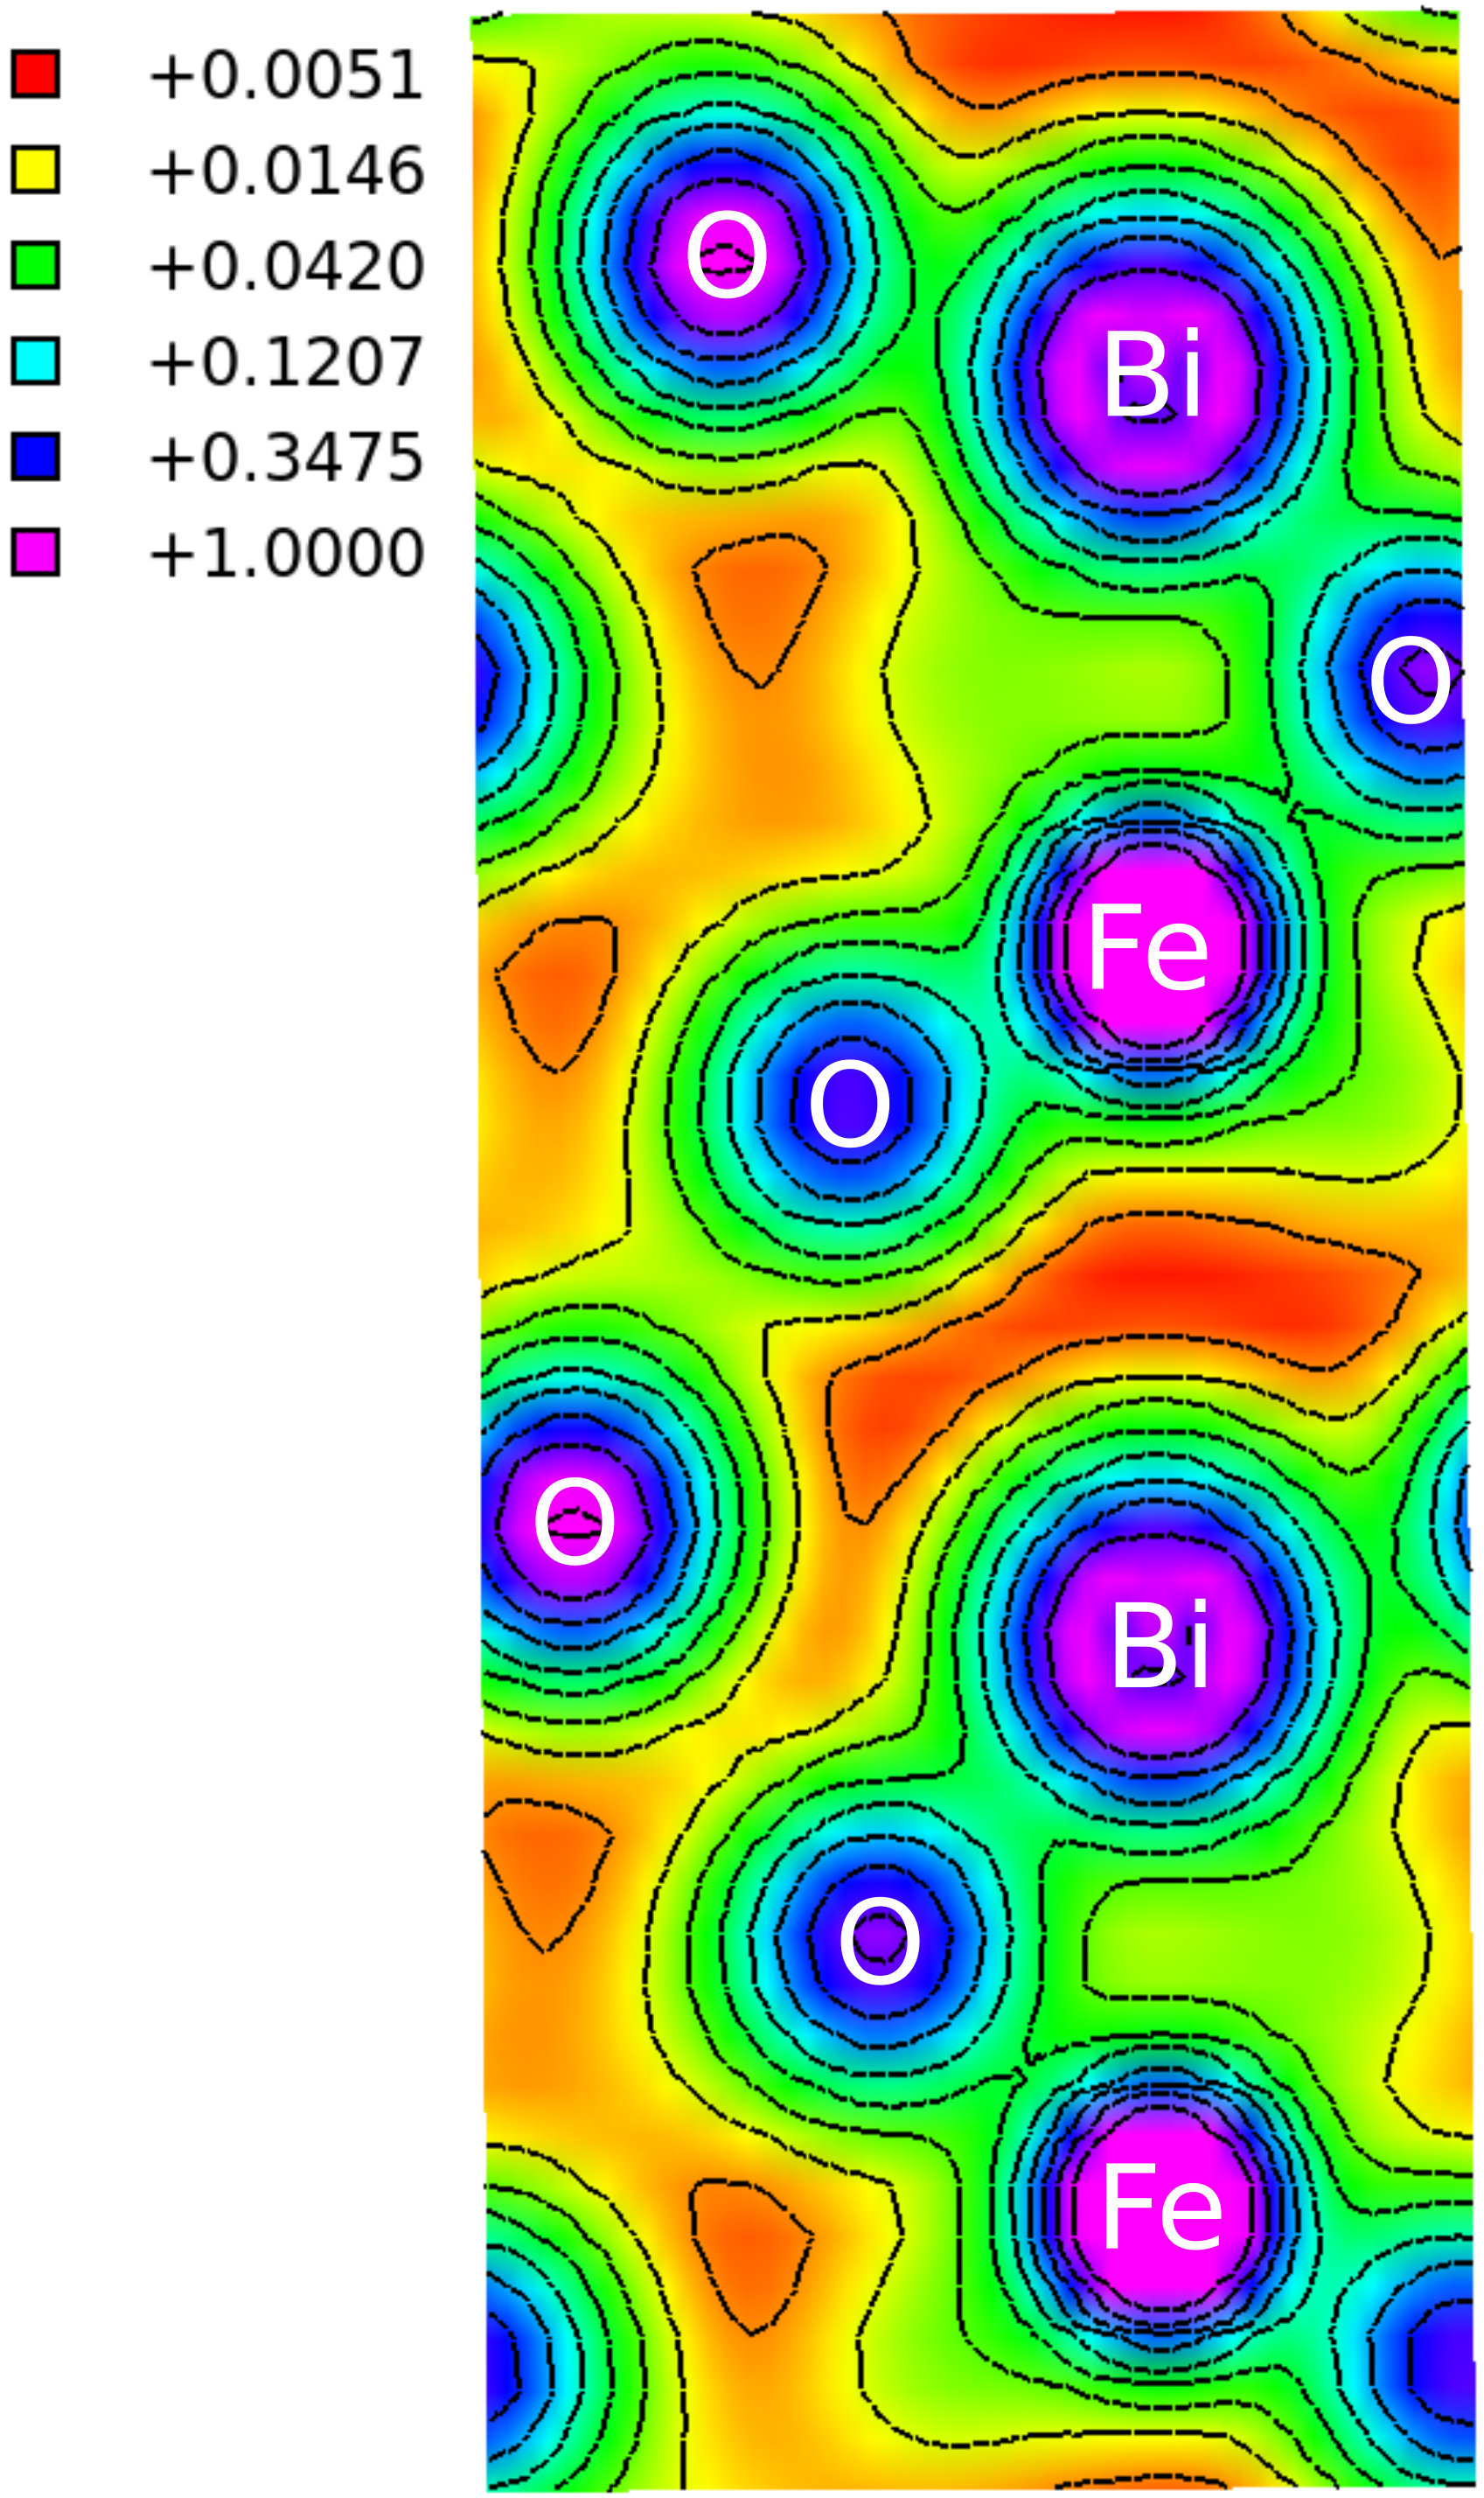
\includegraphics[width=0.4\textwidth]{contenido/resultados/ferrita_bismuto/img_ferrita_bismuto/BiFeO3_DC_plano2_A.png}}
    \subfloat[]{
        \label{bfo_DC_G}
        
        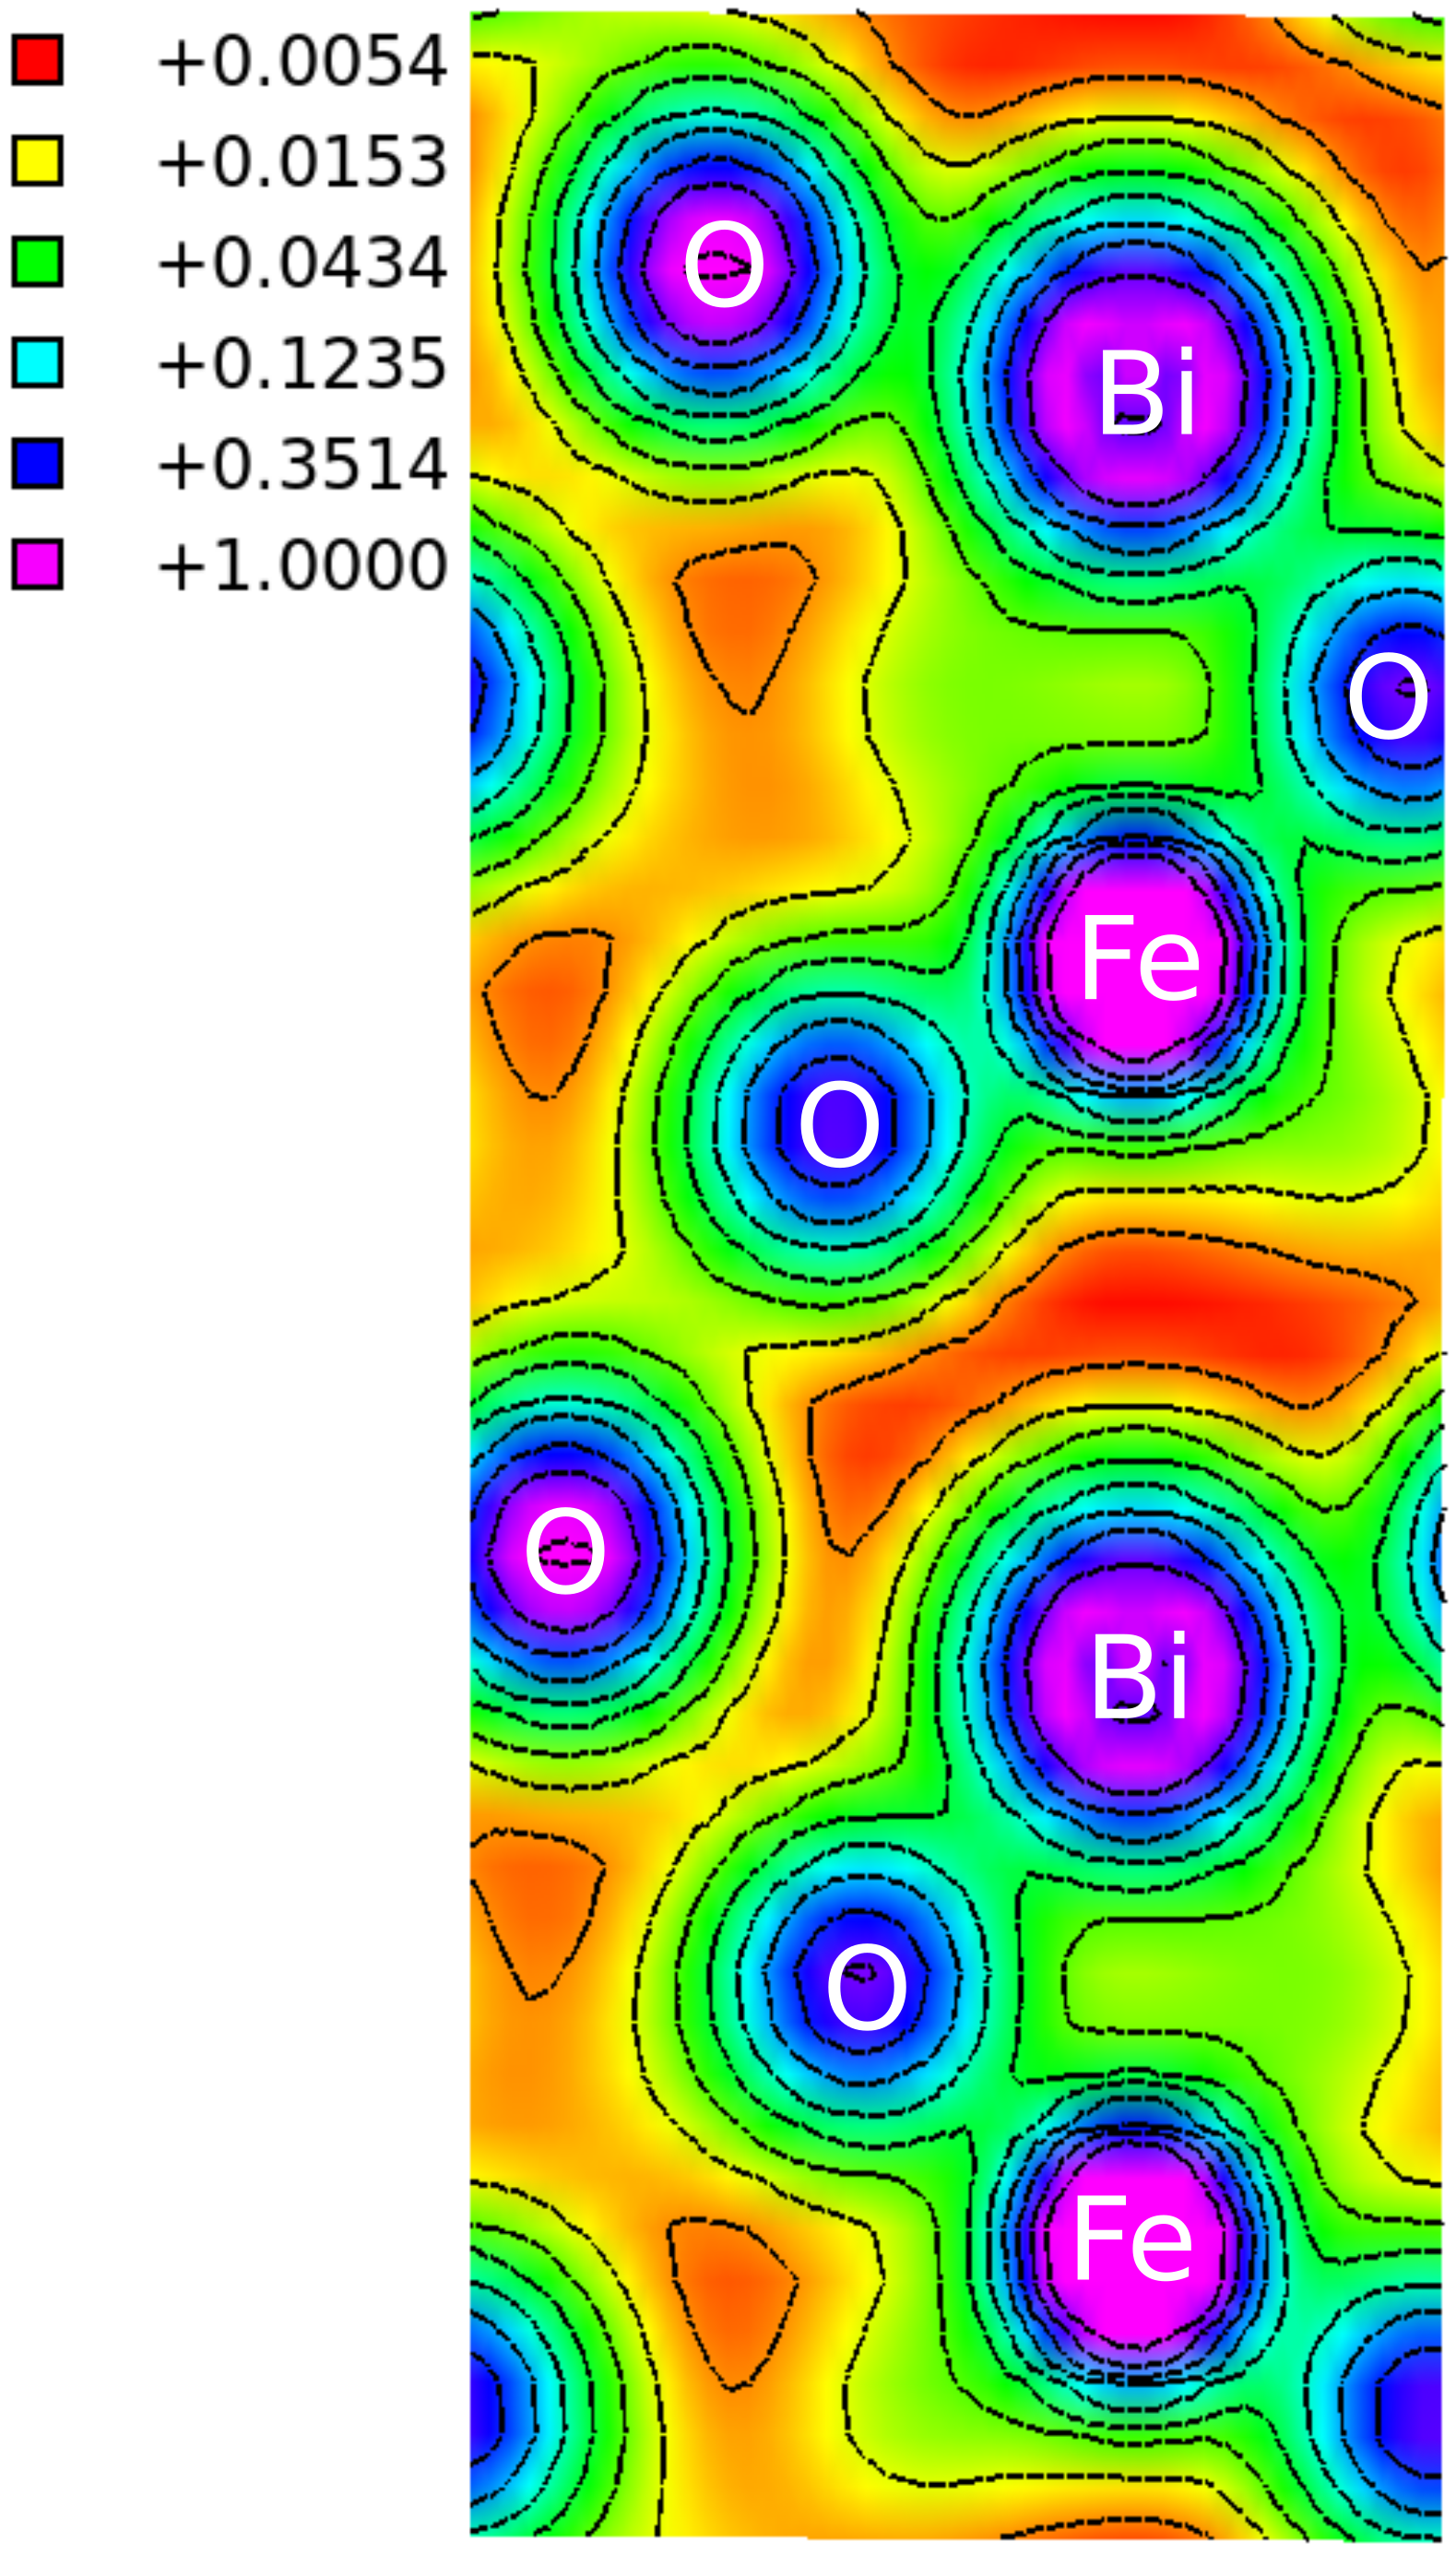
\includegraphics[width=0.4\textwidth]{contenido/resultados/ferrita_bismuto/img_ferrita_bismuto/BiFeO3_DC_plano2_G.png}}
    \singlespace
    \caption[Densidades de carga del $BiFeO_{3}$ con arreglos 
    antiferromagn\'eticos tipo A y G]{\ref{bfo_DC} \subref{bfo_DC_A} Densidad 
    de carga del 
    arreglo 
        antiferromagn\'etico tipo A. \ref{bfo_DC} \subref{bfo_DC_G}  Densidad 
        de carga del 
        arreglo 
        antiferromagn\'etico tipo G.}
    \label{bfo_DC}
\end{figure}